\section{Results}
In this section we present our results from the experiments. The experiments follow the same order as they were presented. 


\subsection{Response time distribution}

%\clearpage
\begin{figure}[h]
    \centering
    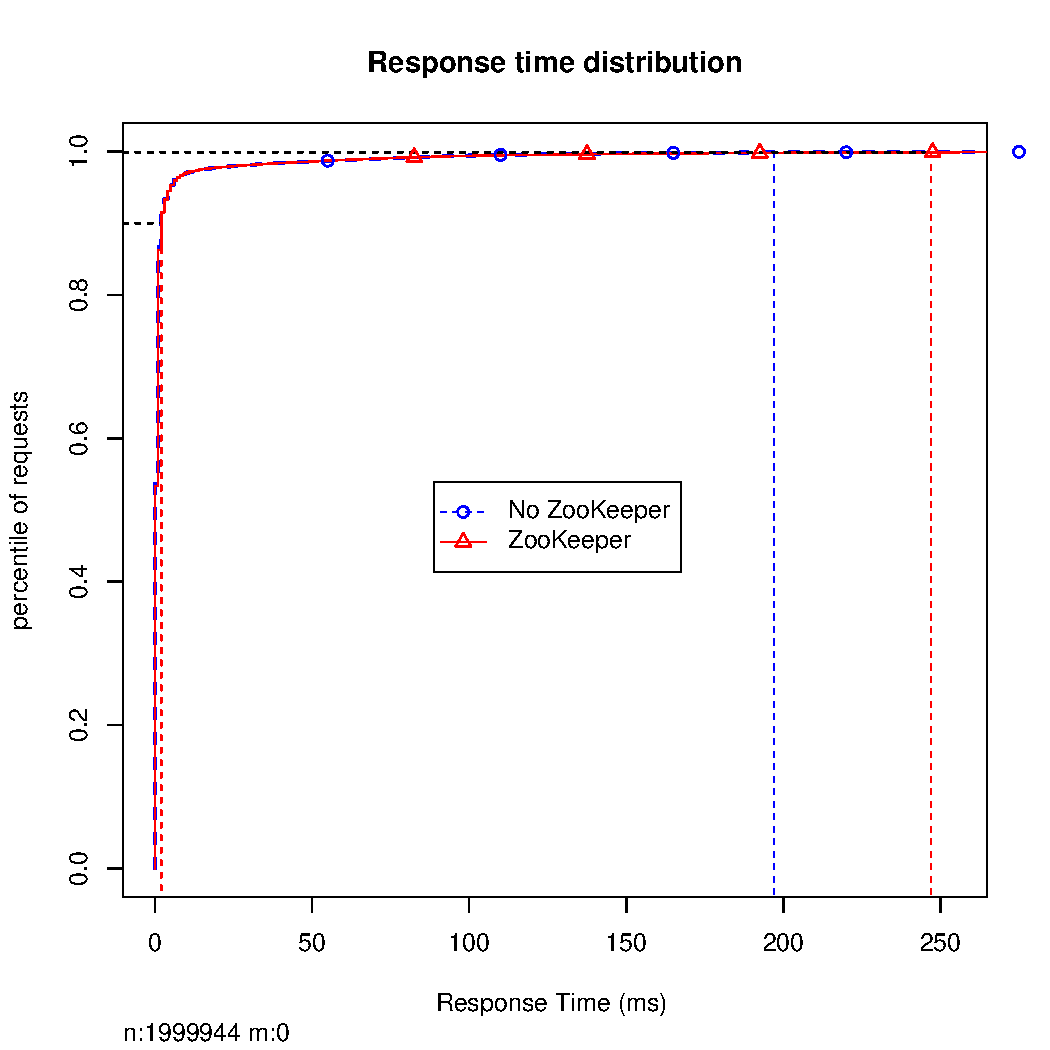
\includegraphics[width=1.0\textwidth]{results/distribution/distribution_macmini}
    \caption{Response time distribution Core 2 Duo Mac mini}
    \label{fig:dist_mini}
\end{figure}

On Figure \ref{fig:dist_mini} we see that both implementations perform similarly on the Mac mini. The vertical lines mark the 0.9 and 0.999 percentile of requests. We see that 90\% of the requests are serviced within 2 ms while at the .999 percentile the response time is at 197 ms for our implementation and 247 ms for the original code.  

\clearpage
\begin{figure}[h]
    \centering
    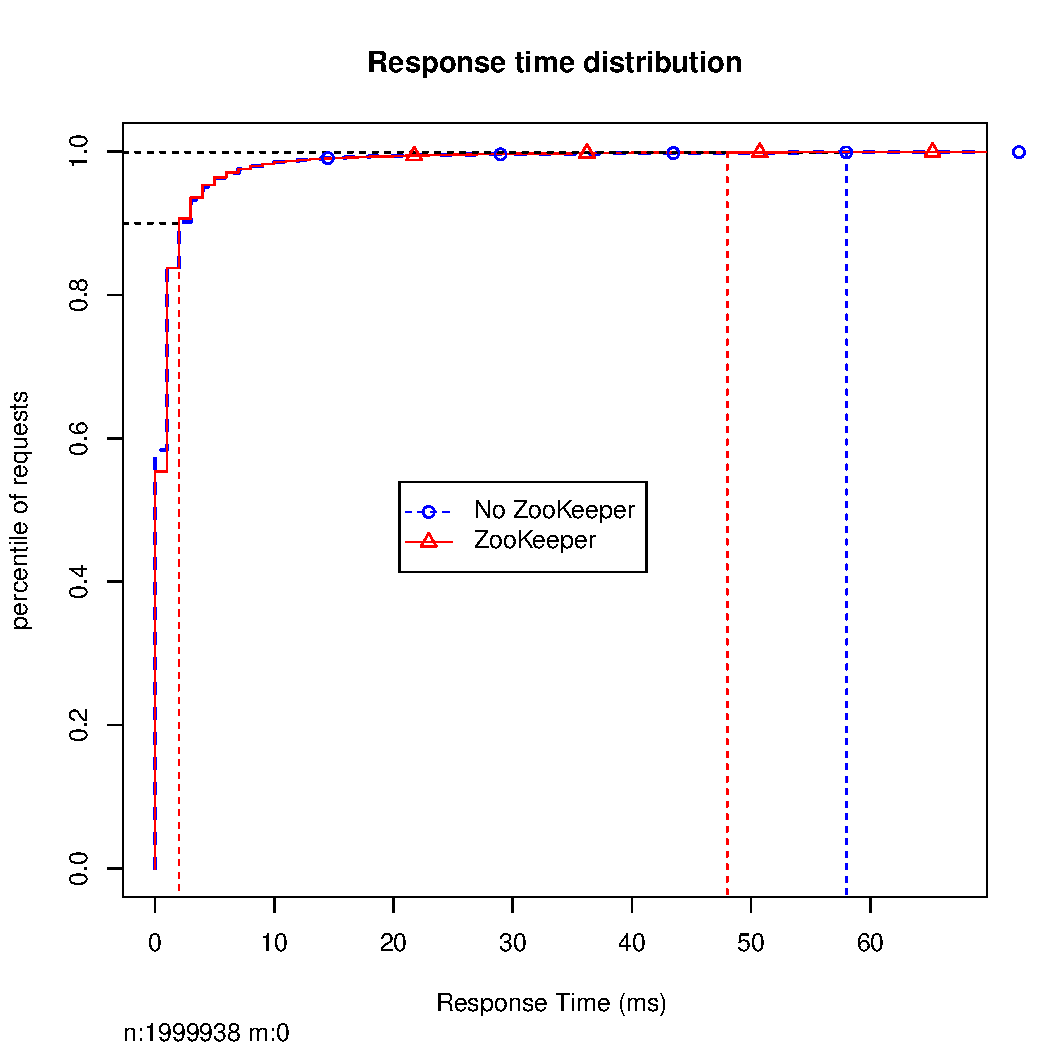
\includegraphics[width=1.0\textwidth]{results/distribution/distribution_knut}
    \caption{Response time distribution i5 MacBook Pro}
    \label{fig:dist_knut}
\end{figure}

On Figure \ref{fig:dist_knut} we see that the i5 MacBook Pro fares better. The vertical lines again mark the 0.9 and 0.999 percentile of requests. At the 0.90 percentile we see no improvement, however at the 0.999 percentile we see a noticeable improvement with 58 ms on our ZooKeeper implementation and 48 ms on the original code.  

\clearpage
\begin{figure}[h]
    \centering
    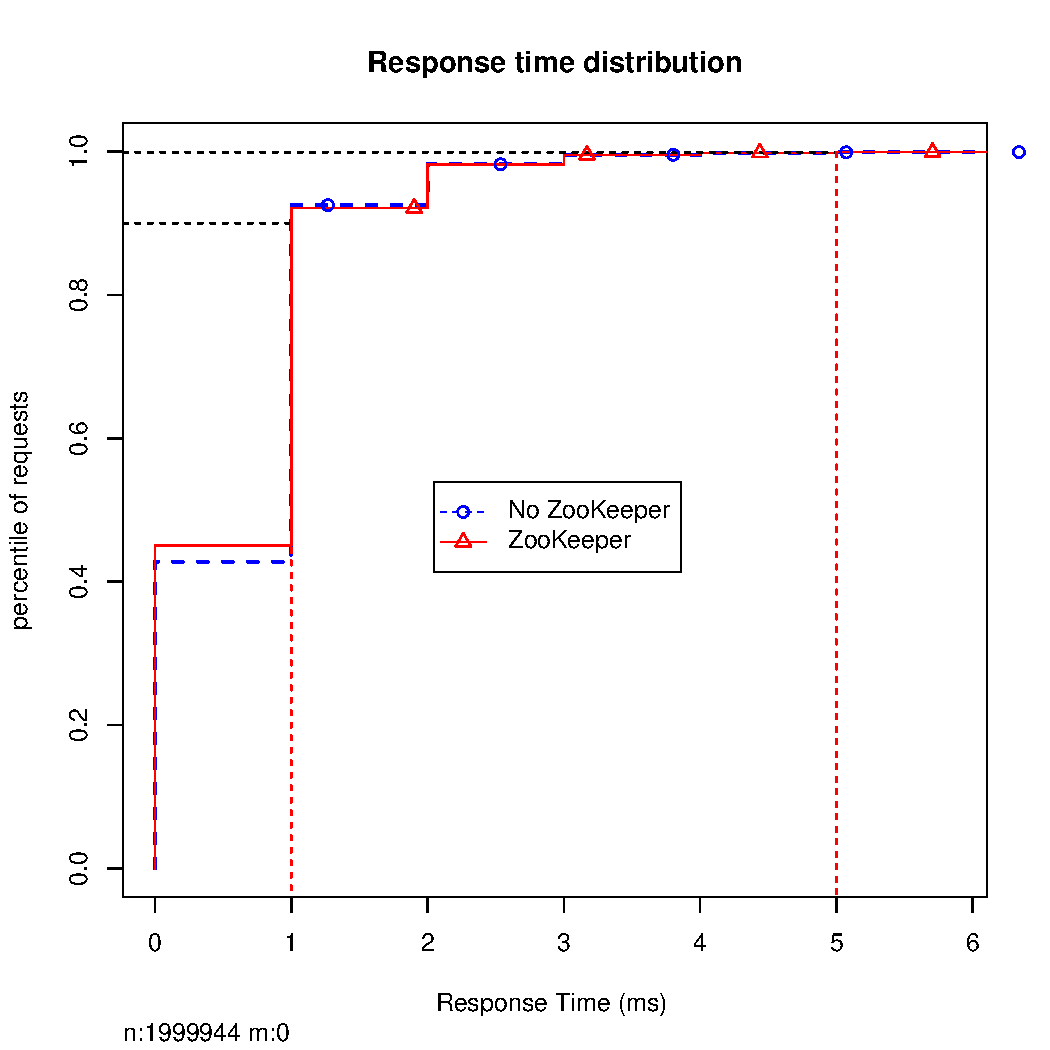
\includegraphics[width=1.0\textwidth]{results/distribution/distribution_eivind}
    \caption{Response time distribution i7 MacBook Pro}
    \label{fig:dist_eivind}
\end{figure}

Finally in Figure \ref{fig:dist_eivind} we see the results on the i7 Macbook Pro. At the 0.90 percentile the system responds in 1 ms in both cases and again we see a great increase in performance at the 0.999 percentile with 5 ms for both systems.

\subsection{Throughput}

\clearpage
\begin{figure}[h]
    \centering
    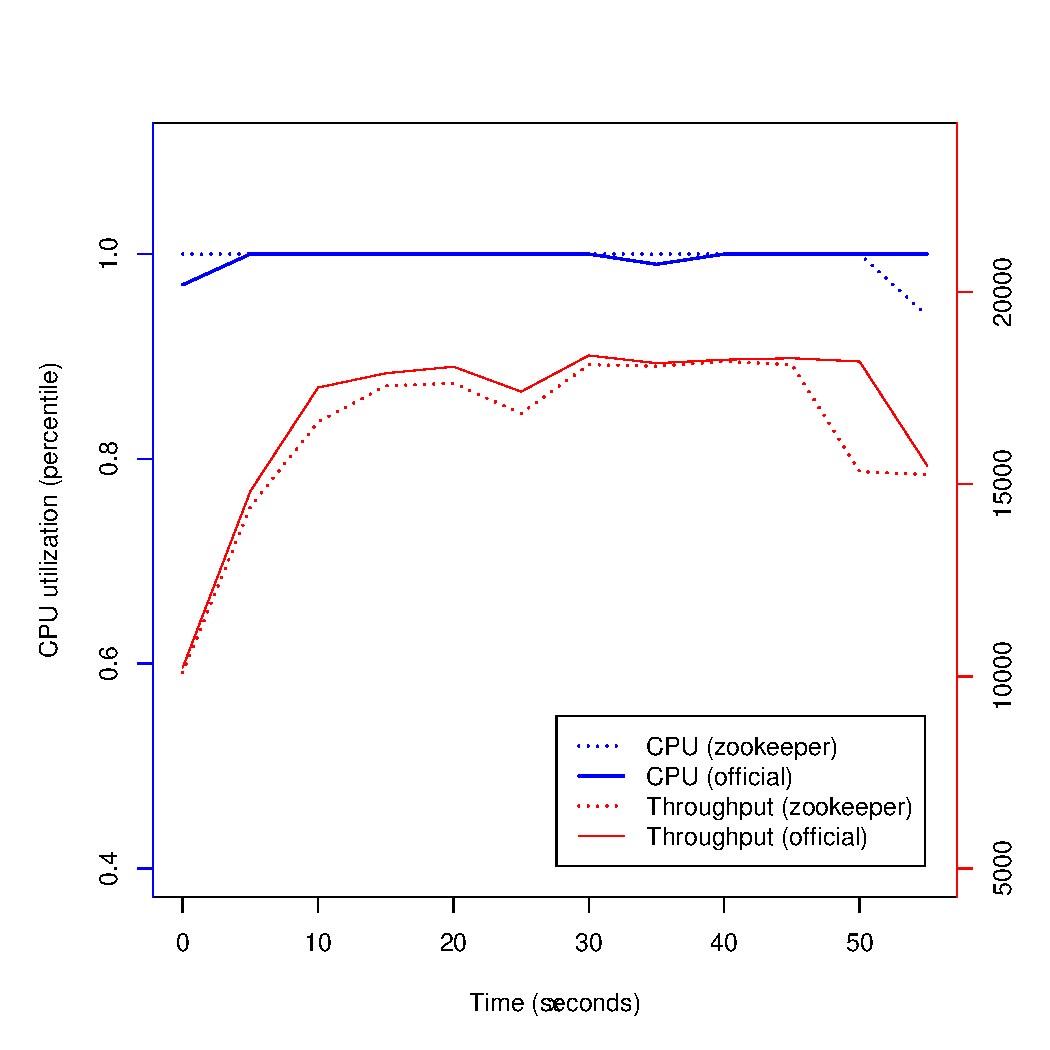
\includegraphics[width=1.0\textwidth]{results/throughput/singlenode/throughput_macmini}
    \caption{Throughput and CPU-load under stress test on Mac Mini}
    \label{fig:thug_mini}
\end{figure}

On Figure \ref{fig:thug_mini} we see that the Mac Mini's Core 2 Duo is clearly running at maximum capacity keeping up with the workload, running at close to 100\% utilization of the CPU. Maximum throughput is hovering around 17k requests per second. 

\clearpage
\begin{figure}[h]
    \centering
    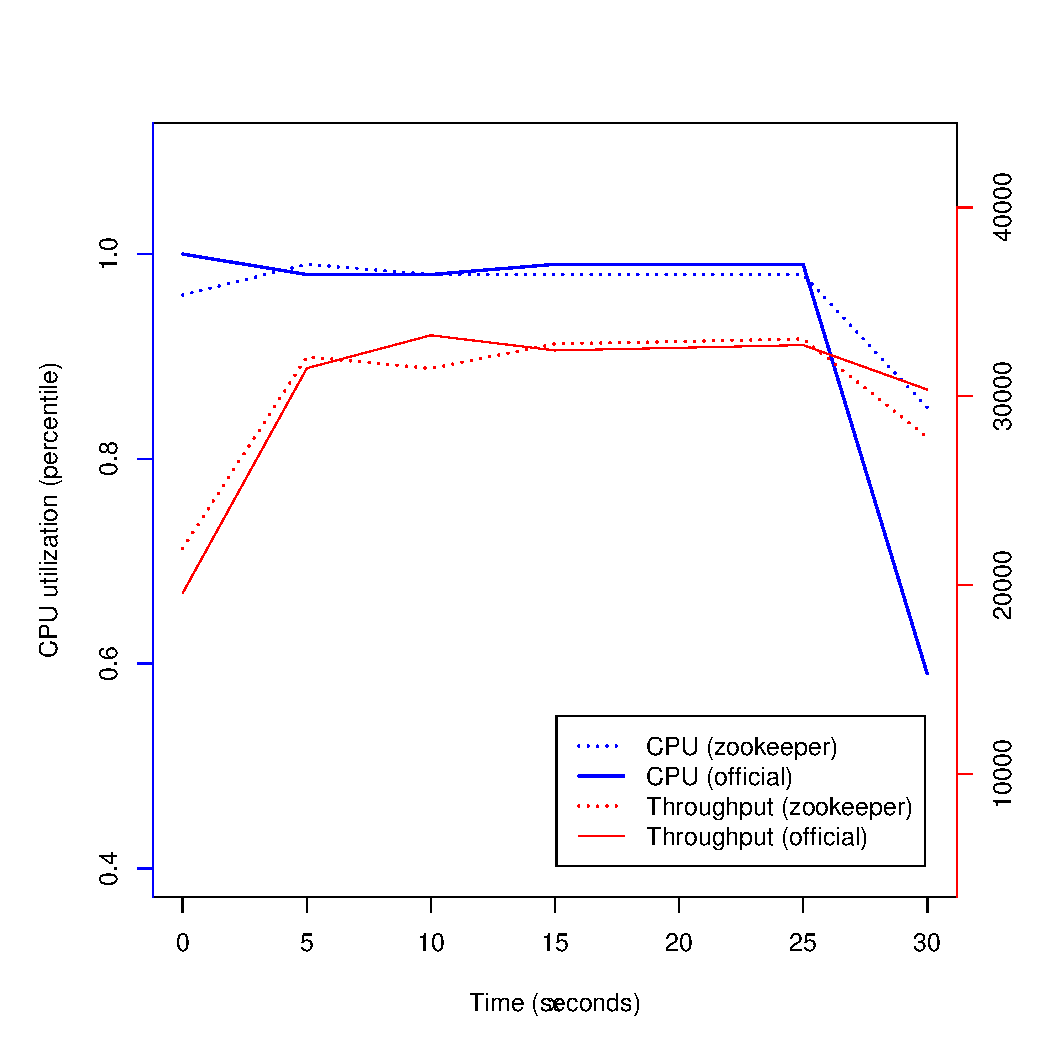
\includegraphics[width=1.0\textwidth]{results/throughput/singlenode/throughput_knut}
    \caption{Throughput and CPU-load under stress test on i5 MacBook Pro}
    \label{fig:thug_knut}
\end{figure}

Figure \ref{fig:thug_knut} paints a very similar picture. The Core i5 in the MacBook performs a lot better than the Mac Mini, but it is still not able to keep up with the workload. It reaches saturation at around 32k requests per second. 

\clearpage

\begin{figure}[h]
    \centering
    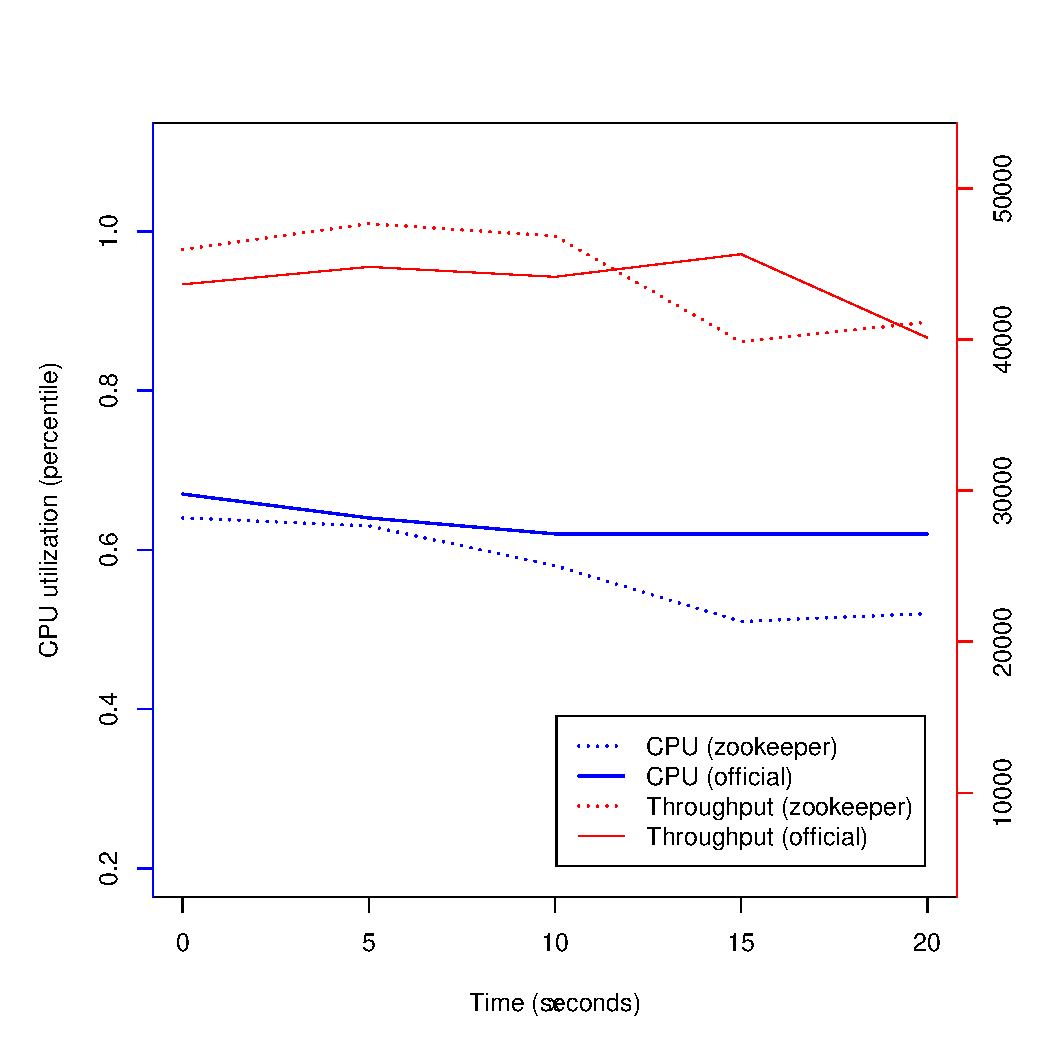
\includegraphics[width=1.0\textwidth]{results/throughput/singlenode/throughput_eivind}
    \caption{Throughput and CPU-load under stress test on i7 MacBook Pro}
    \label{fig:thug_eivind}
\end{figure}

Finally we have the Core i7 Macbook. Figure \ref{fig:thug_eivind} shows us the Core i7 saturated at around 44k requests per second. It is worth noting that in this experiment the CPU-utilization is at less than 80\% meaning there is another factor limiting the system. Our explanation is that disk access might act as a bottleneck and thus limiting the i7 at 44k requests per second.


\clearpage
\subsection{Adaptive cluster behavior}
In this section follows the results form our adaptive cluster experiments.

\begin{figure}[h]
    \centering
    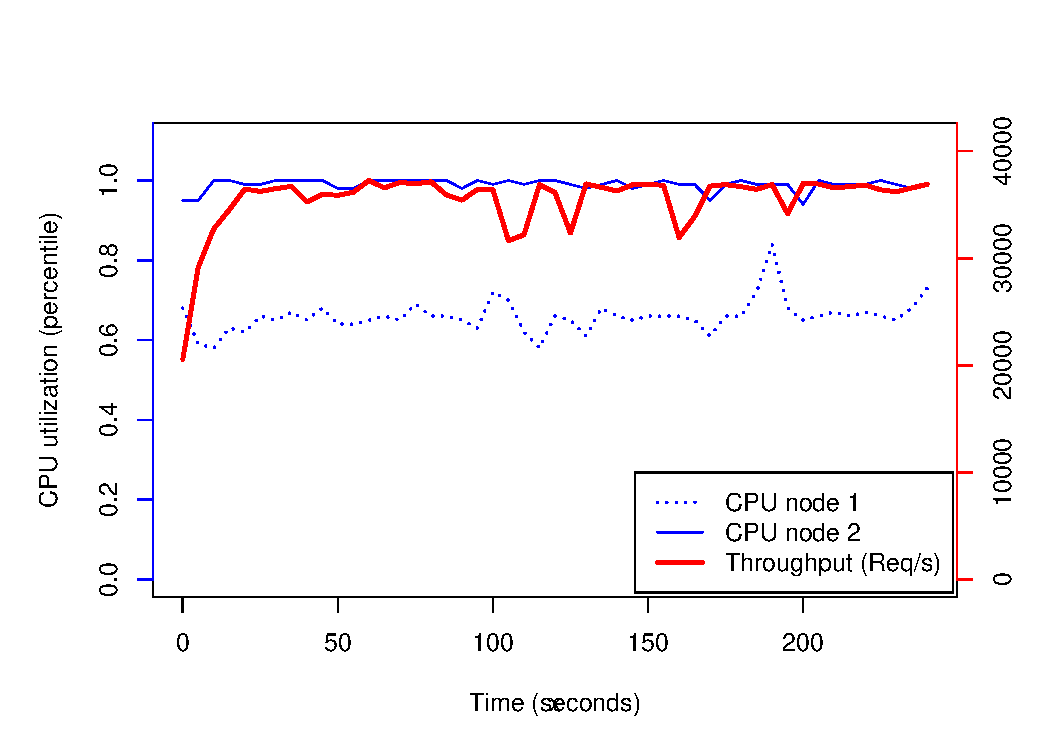
\includegraphics[width=1.0\textwidth]{results/baseline_slowpro_mini}
    \caption{A baseline benchmark for a cluster of 2 nodes serving queries.}
    \label{fig:adaptive_base}
\end{figure}

In Figure \ref{fig:adaptive_base} we see a cluster of 2 nodes serving queries and their CPU utilization. The average throughput for these two is 36k requests/s, yet their individual performance is at 17k and 33k, respectively. We can also note that the CPU of node 1 is bound around 64\%, where as node 2 is at above 95\% the entire run.

\clearpage
\begin{figure}[h]
    \centering
    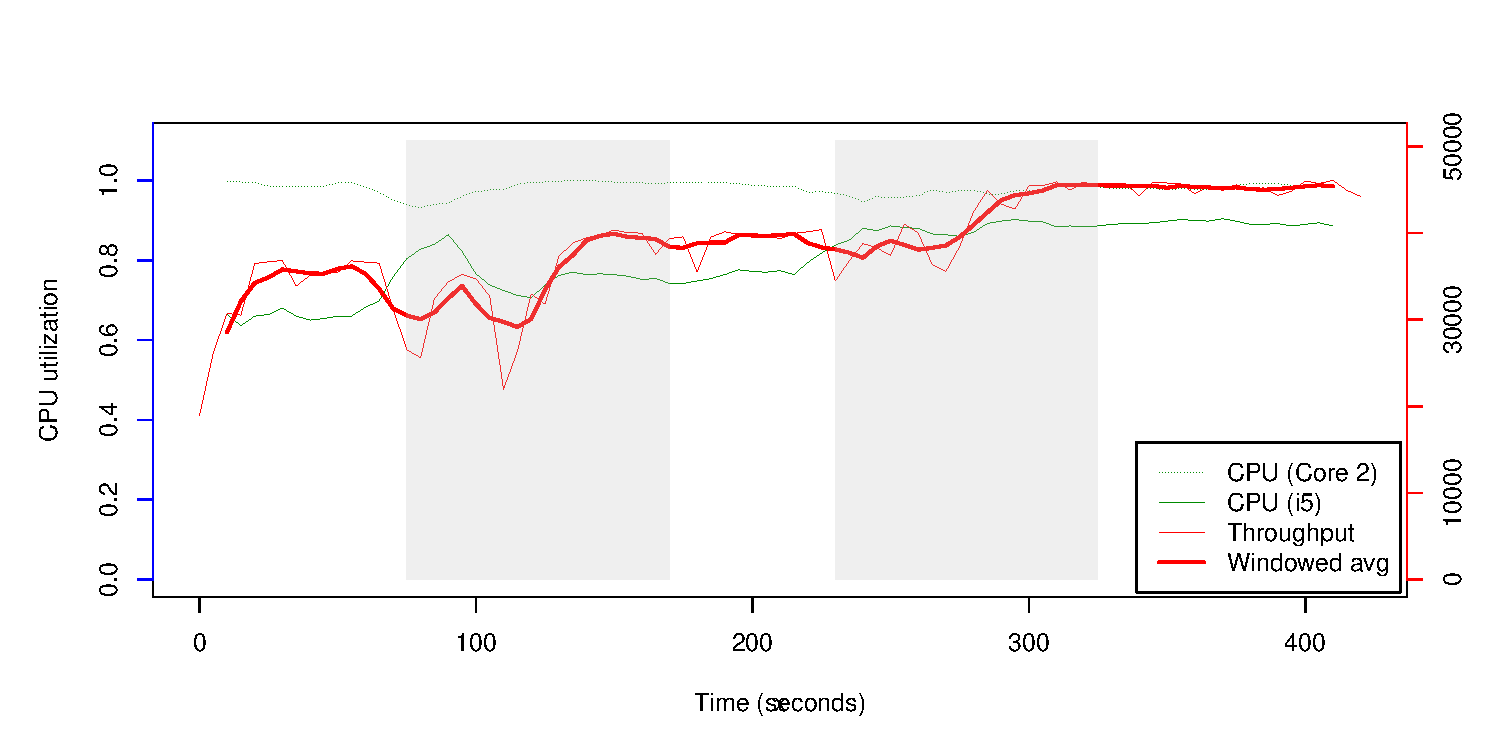
\includegraphics[width=1.2\textwidth]{results/rebalance_manual_2node}
    \caption{Manual moving of 2 partitions from a struggling node (Core 2). Grey regions mark rebalance period, where data is prepared and transferred.}
    \label{fig:adaptive_man}
\end{figure}

In Figure \ref{fig:adaptive_man} we see 2 manual rebalances. We see total CPU-utilization increase as we move partitions away from a struggling node and over to one less worked. The aim of this experiment was to get a baseline to compare our automatic rebalance service to. We see throughput steadily increase after each rebalance moving from around 36k up to 45k. During the rebalance we have two very distict drops in throughput. The first one is from when request starts being proxied and all client threads must reconnect. The second one is from the actual data transfer. 

\clearpage
\begin{figure}[h]
    \centering
    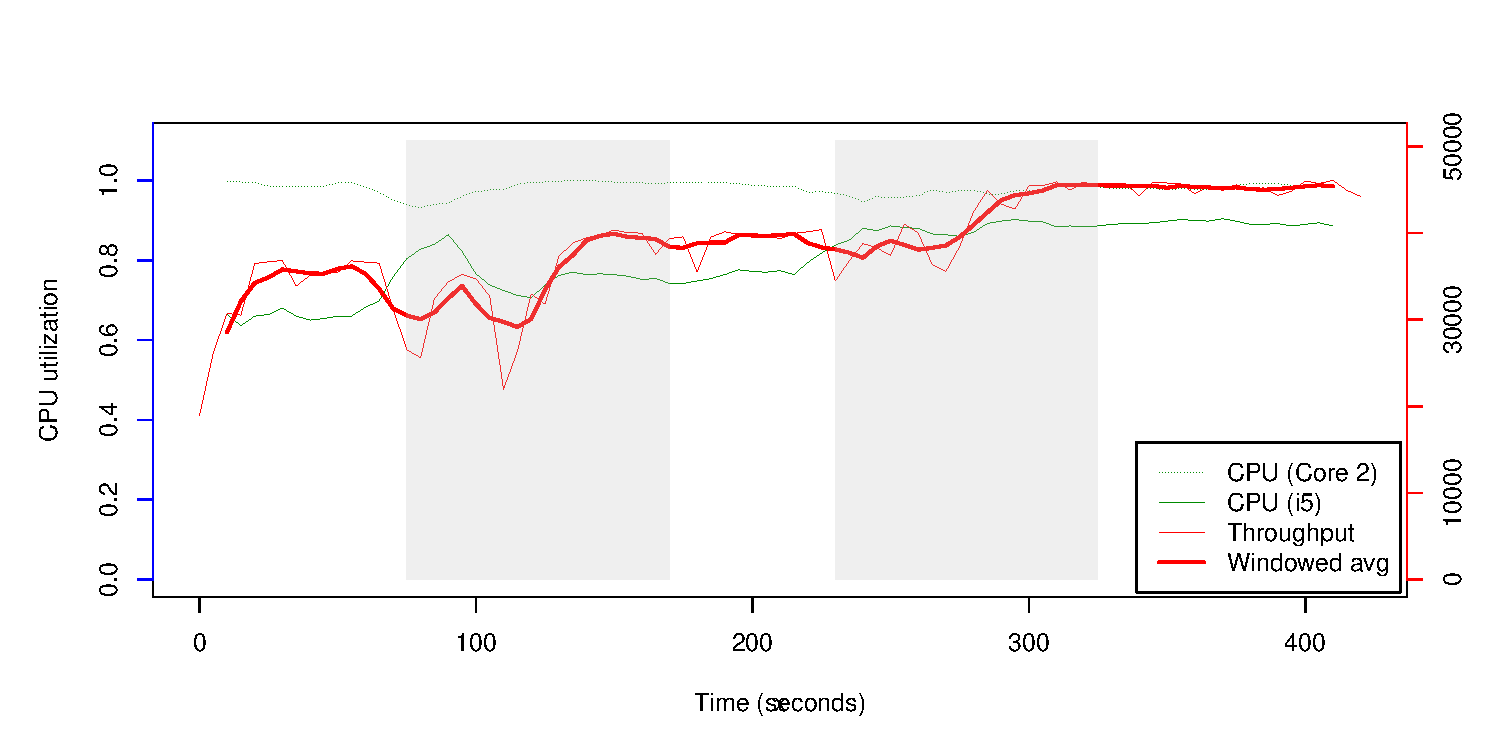
\includegraphics[width=1.1\textwidth]{results/rebalance_auto_2node}
    \caption{Automatic moving of 2 partitions from a struggling node (Core 2). Grey regions mark rebalance period, where data is prepared and transferred. CPU threshold set at \texttt{0.84}.}
    \label{fig:adaptive_auto}
\end{figure}
Figure \ref{fig:adaptive_auto} shows the same experiment just automated by Headmaster. We again see a steady increase in throughput as partitions are moved. We start out at about 36k requests per second, moving up to ~46k requests/s as the load balances out. Also here we see two dips in performance per rebalance period. The first one stems from the clients reconnect after new metadata is discovered. The second one is during the moving of records between nodes.

\clearpage
\begin{figure}[h]
    \centering
    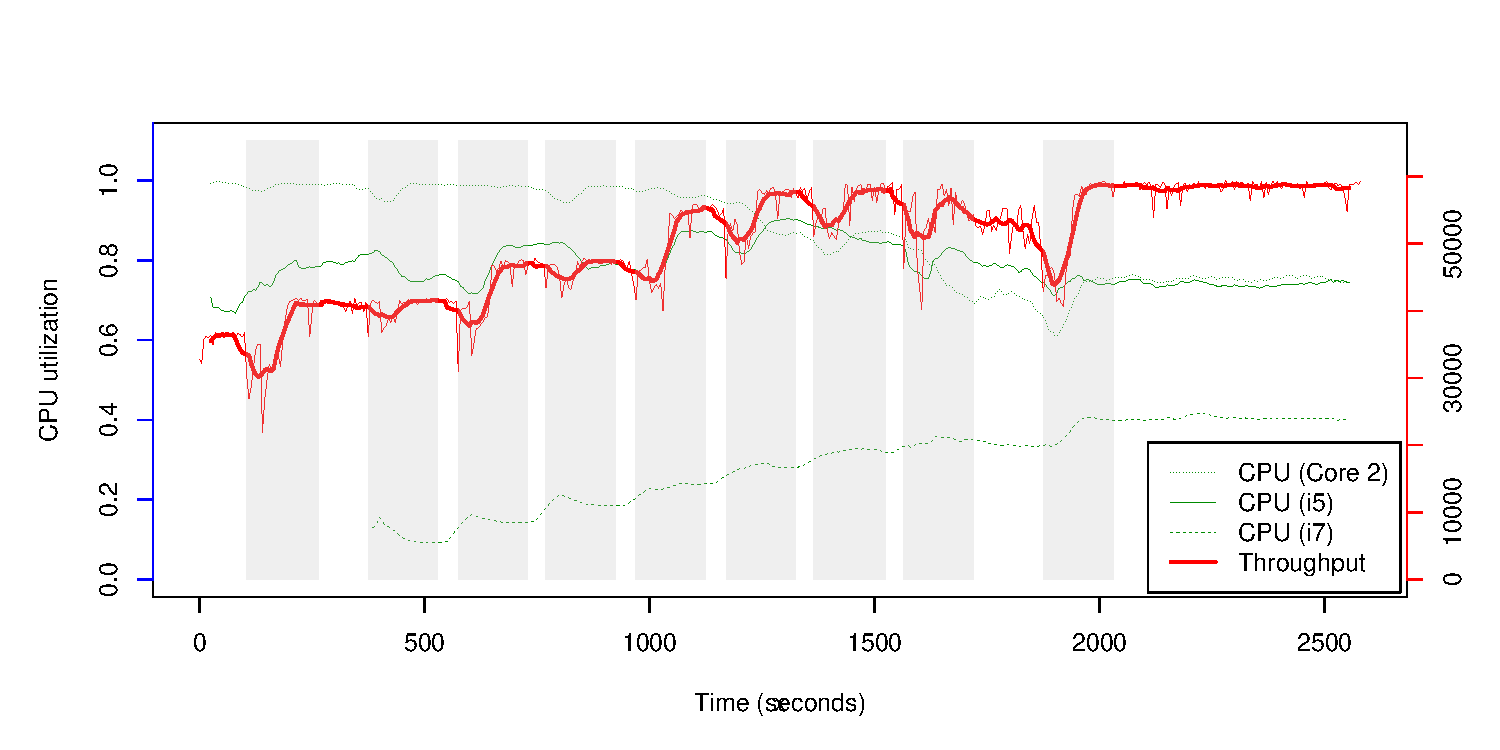
\includegraphics[width=1.0\textwidth]{results/adaptive3node}
    \caption{Automatic migration of partitions in a struggling cluster after a third node joins. A smoothed average is plotted on top of throughput, but is excluded from the legend for spatial reasons.}
    \label{fig:adapt_3node}
\end{figure}
Figure \ref{fig:adapt_3node} shows the result adding a node to a struggling cluster and rebalance live. At t=380 the i7 is introduced to the cluster. We see a steady increase in performance as more and more partitions are moved to the i7. In the end the different nodes are holding different number of partitions. This is 3,5,8 for the Core 2, i5 and i7 respectively. 

At t=1700 there is a significant loss of throughput after a rebalance. We found no reason for this in our logs, so we suspect this to be related to unrelated work done by the operating system on the workload generating computer, but we failed to find any verification on this. The test is quite long, running for over 40 minutes and a quite a few of our tests got affected by random events on this time frame.

\clearpage
\begin{figure}[h]
    \centering
    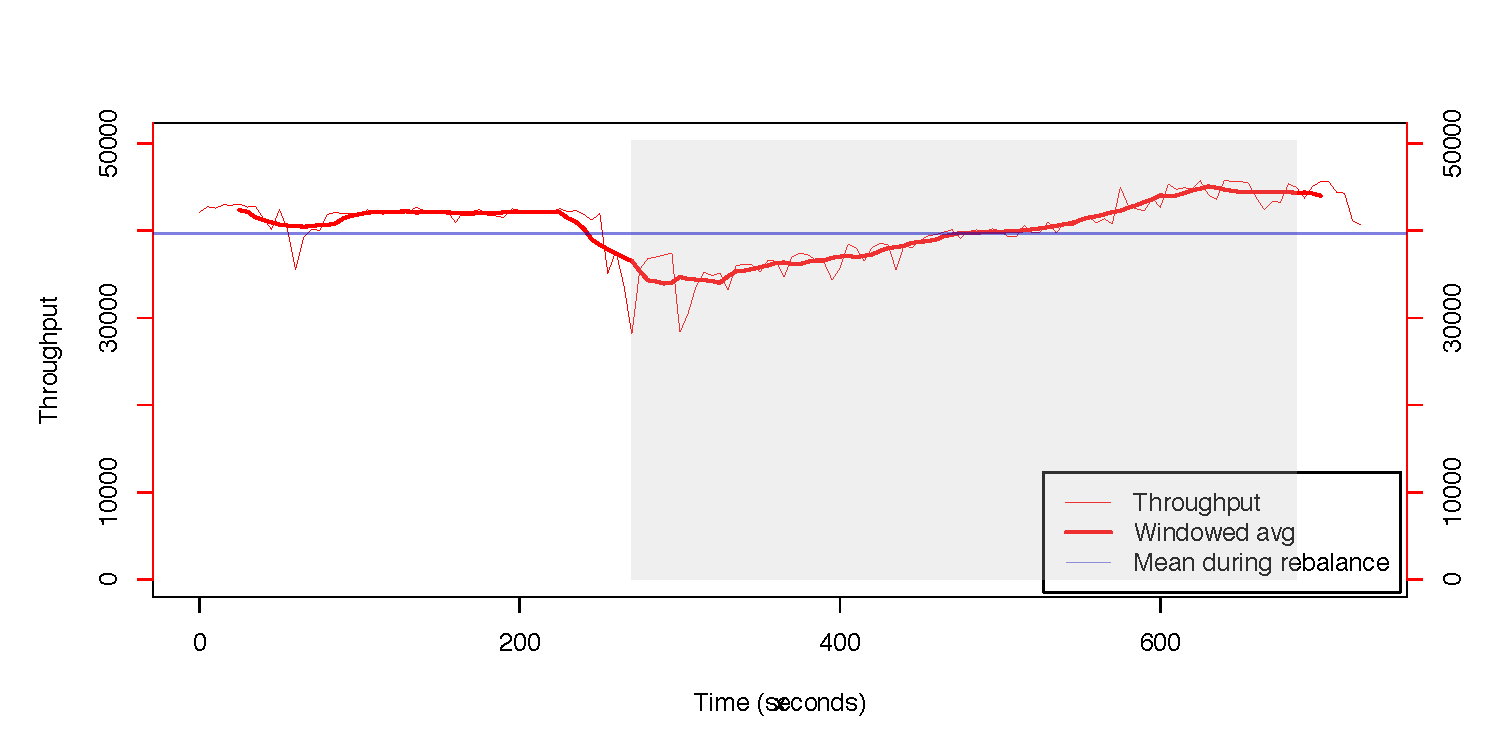
\includegraphics[width=1.0\textwidth]{results/throughput/adaptive/zookeeper/auto_3nodes_muchdata_wow}
    \caption{In depth view of thoughput during a big rebalance operation. The blue vertical line marks average throughput during the rebalance.}
    \label{fig:adapt_big_rebalance}
\end{figure}

Figure \ref{fig:adapt_big_rebalance} shows a large partition being moved. The partition holds almost 1 million entries or almost 1 gigabyte of data. Before the rebalance we have a steady throughput of 42k requests per second. For the duration of the rebalance, we average around 39,5k requests per second. We move a around 6\% of all values and the rebalance causes a 6\% loss of throughput, running at roughly 94\% of performance before the rebalance. 

Contrary to our expectations, we have a sudden drop in throughput followed by a steady increase during the rebalance. The sudden drop is caused by all clients being forced to fetch the newest metadata. The steady increase in throughput is a result of an increasing number of the entries being available at the stealer node, and lessening the need for proxying GET requests.

\clearpage
\begin{figure}[h]
    \centering
    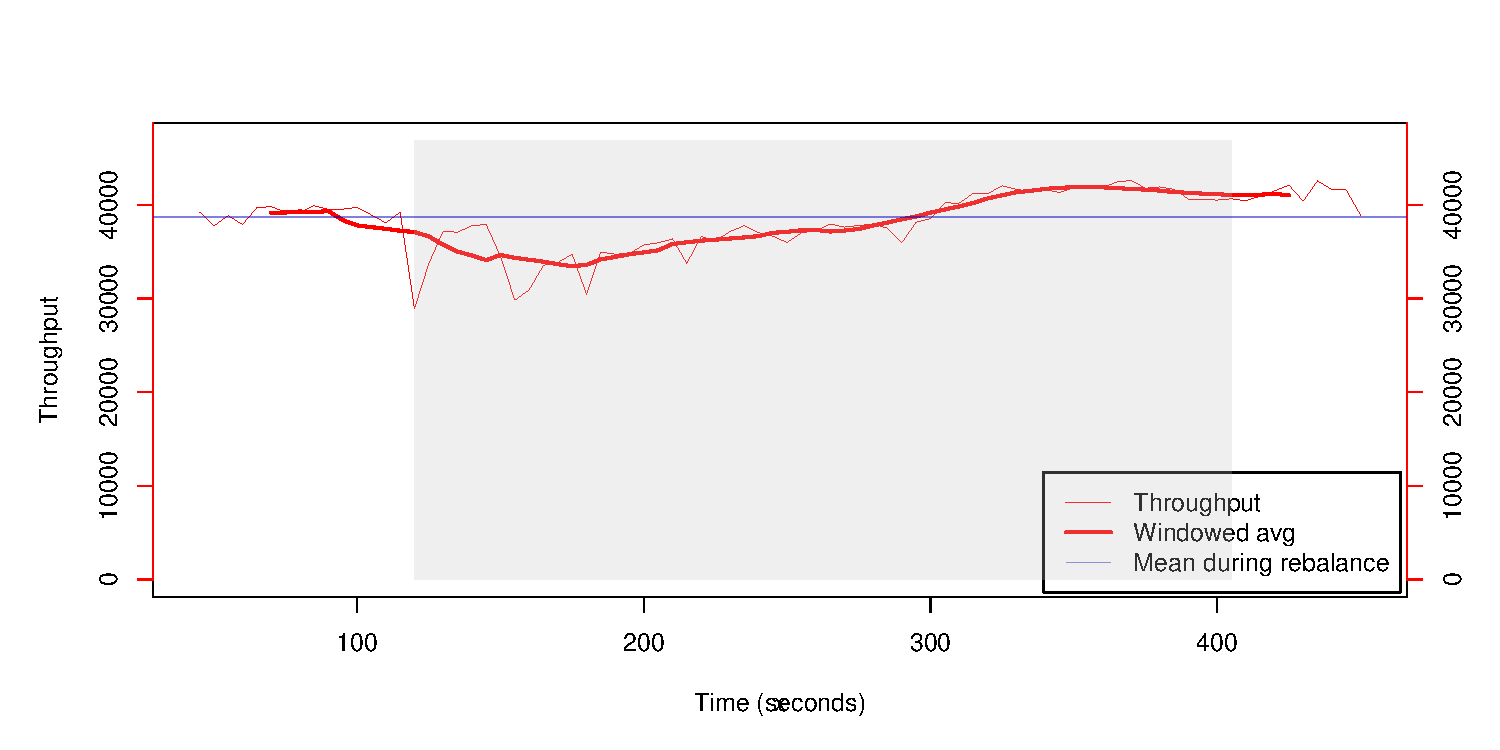
\includegraphics[width = 1.0\textwidth]{results/throughput/adaptive/zookeeper/auto_3nodes_32part.pdf}
    \caption{In depth view of thoughput during a rebalance with 15 million entries and 32 partitions. The blue vertical line marks average throughput during the rebalance.}
    \label{fig:adapt_small_rebalance}
\end{figure}

In Figure \ref{fig:adapt_small_rebalance} we see the results of moving one of the 32 partitions. Before the rebalance we service 39,2k requests per second, while during the rebalance we average 38,6k requests per second. This shows that over 98\% of the cluster performance is maintained during the process. For comparison we now move 3\% of all values.


